\documentclass[../../../OAE-SPEC-MAIN.tex]{subfiles}
\begin{document}

 \section{RISC Protocol Design: LIVENESS (Knowledge)}

\begin{fullwidth}
 \begin{figure}
 
\includegraphics[width=1.6\linewidth]{./figures/First-Slice-Encodings.pdf}
\end{figure}
\end{fullwidth}

%\vspace{6pt}
\sidenote{\textit{First Slice: \texttt{CONTEXT} (Packet Mission). All bits are green (owned and written by Alice)}}
%\end{fullwidth}

%
%\begin{fullwidth}
%  \begin{center}
%    \includegraphics[width=\linewidth]{../.././figures/First-Slice-Encodings.pdf}
%  \end{center}
%  \marginnote[Figure: A full-width figure with its caption placed in the right margin.]{Figure: A full-width figure with its caption placed in the right margin.}
%\end{fullwidth}


\subsection{Bipartite Link}

There are exactly two parties on the DAE Link. We could call them \texttt{alice} and \texttt{bob}. We prefer to call them self and not self. From Alice’s perspective, she knows her own identify, but she does not know the identity of the party she is communicating with (yet). We aim to achieve mathematical precision in our specifications. This will be important when we wish to formally verify the scouting, routing, and cluster membership protocols. It will be critical also in formally verifying confinement properties of the trees above.

The encoding supports Intanglement (hidden circulating events internal to the link) and Extanglement (Atomic Token Passing through the link (Newtons cradle). These protocols obey the mathematics of mutual information, and provides some of the properties of quantum entanglement, such as superposition, conservation of information, and no-cloning. We use these properties to provide our protocols with a clear notion of simultaneity (through the synchronization of mutual information), and guarantee atomicity for transaction protocols through conserved quantities which in-turn guarantees exactly once semantics (EOS).

Conventional L2 \& L3 networks rely on redundancy, repetition and rerouting, in multipartite (1:N) relationships. Which was necessary when information is disseminated (transmitted blindly hoping the receiver catches it). When information can also be synchronized, by a Tx/Rx—T/Rx loop on a bipartite Ethernet link, we can employ Pseudo Entanglement: A form of temporal intimacy, where bits shared in a circulating frame can exploit the same mathematics, (but not the full quantum properties) of Entanglement. This insight allows us to engineer a clear notion of simultaneity, and exploit a classical version of the no-cloning theorem to achieve the holy grail in distributed systems and database isolation: exactly once semantics.

\subsection{Link Engine}

Alternating Causality (AC) is the name we give to the initialization, maintenance and tear down of Common Knowledge (CK) in the Link. Experience with modern SerDes designs leads us to an 8 byte slice architecture for a “minimum irreducible” CK protocol. Symmetry demands that we use half (4-bytes) for \texttt{alice} (what I know about me) and the other 4-bytes for \texttt{bob} (what I know about you). Three packet exchanges get us from initialization (both sides know nothing about each other) to the “I know that you know that I know” (IKT YKT IKT) equilibrium state for basic liveness. \marginnote{It takes a while to gain an intuition for this issue of causality, based on the physics. For now, please accept that this is way of doing things is essential and enables a rich set of transaction types to be built on top, all with immunity to link hazards.}

We don’t use classical (increment only) clocks, counters, or timers in the link. Instead, we use balanced ternary arithmetic [1] The digits of a balanced ternary numeral are coefficients of powers of 3, but instead of coming from the set {0, 1, 2}, the digits are {-1, 0 and +1}. They are balanced because they are arranged symmetrically about zero.  We use this symmetry to manage the direction of causality (is alice the initiator of causal flow sending tokens to bob, or the receiver in causal flow receiving tokens from bob?).  This becomes important as we go up the protocol stack and construct reversible subtransactions.  

We extend the simple ternary arithmetic with plus and minus zero. {-1,-0,+0,+1}. This enables the protocol to differentiate between the posibits and negabits [2], with an ancilla control over the intended direction of the next operation (positive or negative). This is used to control the direction of the state machine when recovering from errors.

Intanglement is enabled by reserving 4 bits in the frame for CK (2 bits for Alice, 2 Bits for Bob). One message will let Bob know about Alice.  A second message lets Alice know that Bob knows, the third message lets Bob know that Alice knows that Bob Knows, consistent with both Moses and Halpern version of CK, and the Spekkens Knowledge Balance Principle (KBP).
Time, inside the link moves forward when packets arrive. Time moves backwards when packets depart. It doesn’t matter how many times a packet bounces around, time goes forward only when it is received by one end of the link and it stays (is absorbed). Information is then turned into Knowledge. 

In a similar way to two phase locking, Link CK can be extended from 2 Ternary bits (Trits) to any number. Since we are using 2 binary bits to encode one Trit, we posit that the set of 2-message exchanges to synchronize them is 1, 2, 4 and any multiple of 4. This observation drives the encoding for the State Machine Engine, Described below.
Our Protocol is based on \href{https://wiki.xxiivv.com/site/reversible_computing.html}{Reversible Computing}. 

 \begin{marginfigure}
 \centering
  \includegraphics[width=1.1\linewidth]{./figures/First-Slice-Encodings.pdf}
\caption{\centering First Slice: CONTEXT. Least significant 32 bits of  transmitted packet.}
\end{marginfigure}

\subsection{Slice Engine}
The core of the Æ protocol is the Slice Engine. The first slice (or pre-frame slice) determines the packet mission, and carries the alternating causality for the Link State Machine (LSM).

Each 64-bit slice represents an atomic delivery of bits on the wire from the SerDes. Typically 2 slices will be sent back to back and the Slice Engine must be prepared to receive both, although the receiver may decide to pre-empt the frame in its immediate response to the first slice if it wishes to immediately begin a real data or transaction operation. The second slice will be on its way, and its Error Detection Byte must be evaluated before forwarding on other ports (with the exception of the port it was received on, which is the entanglement mechanism).

\begin{marginfigure}
\centering
%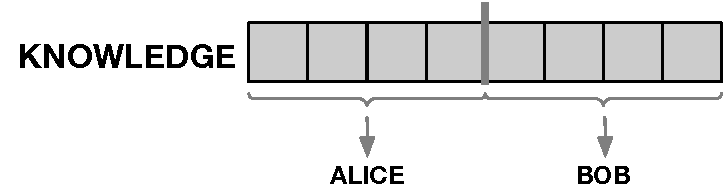
\includegraphics[width=1.15\linewidth]{.././figures/knowledge.pdf}
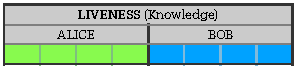
\includegraphics[width=1.05\linewidth]{./figures/LIVENESS.pdf}
\caption{\centering One Byte Provides Knowledge }
\vspace{10pt}
\end{marginfigure}


 \begin{marginfigure}
 \centering
  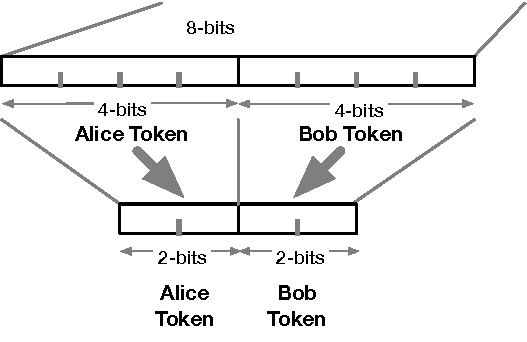
\includegraphics[width=1.15\linewidth]{./figures/transform1.pdf}
\caption{\centering First Rewriting Rule. Alice Owns and possesses Context Slice}
\vspace{20pt}
\end{marginfigure}




The first slice completely defines the rest of the frame. There are 4 fields: PROTOCOL, LIVENESS, STATE, and TRANSITION.  This is “reflected” from the upper half to the lower half by the receiver, so that only the lower 32 bits are modified, and the upper 32 bits remain unmodified.

The \texttt{PROTOCOL} Byte defines the “mission” of the packet. What each side of the link needs the other side to know about the current frame. 
\texttt{LIVENESS} defines the Temporal Intimacy of the link — whether events on both sides of the link are directly connected or not.

\texttt{STATE} Defines which state machine is currently in use. Can be used as a sanity check in conjunction with Protocol.
Transition  Defines which state in the state machine we are in, and which direction we are going (forward or reverse).

\subsection{General Principles}

Links are constantly interacting, at the slice level, instead broadcasting entire frames (or sets of frames) imposing on the other side and hoping they catch the bits. This provides opportunities for error detection and correction that would otherwise require ECC and FEC. The theory behind this is described in detail in the document “Shannon-Interaction-Machine”. 

The first 4 slices are dedicated to Theseus (scouting protocols). The payload (slices 4-7) contain the Theseus Opcode and parameters — instructions to the scout, including what to do if it encounters an exception (a software or hardware hazard).

When the protocol type is Ariadne (groundplane/trees) the last 4 slices (payload) contains tree-building instructions, such as the CellID of the originator, and the CellID of the Deputy (one hop away from root). This becomes a complete specification for dissemination of the tree without unnecessarily revealing secrets which need to be kept local (confined).

Another protocol type is Icarus (legacy connections to the outside world). This represents a more heavyweight protocol which provides a formally verified TPI (Transaction Processing Interface), which provides significant guarantees, but with costs.

\subsection{General Frame Format}

   \begin{figure}
% \centering
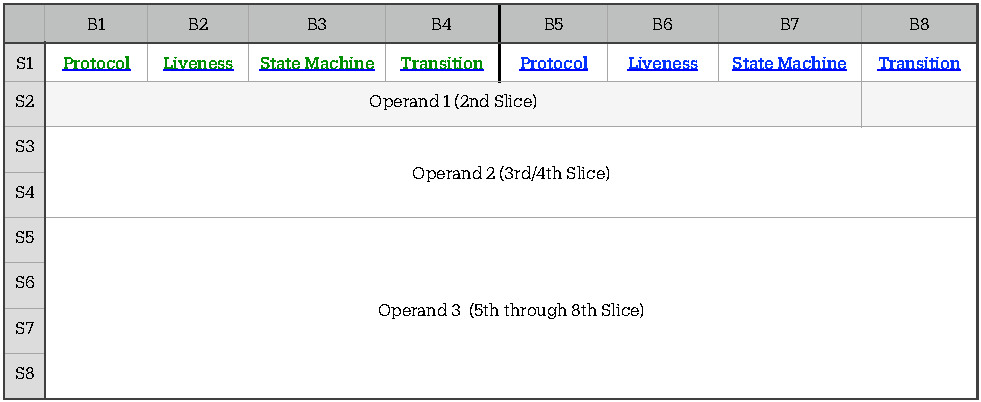
\includegraphics[width=1.5\linewidth]{./figures/General-Frame.pdf}
%  \hspace{20mm} 
%\caption{First Slice:}%\\ The Packet Mission \hspace*{0pt}}
\end{figure}




This protocol is \emph{symmetric}. We describe all operations from the perspective of \texttt{ALICE}, with responses from \texttt{BOB}.


\subsection{Error Detection and Correction}

%%\documentclass[../HFT-main.tex]{subfiles}

%\usepackage{currfile}  % <— key line

\title{Error Detection/Correction philosophy}


% ----------------------------------------------------
% 1.  Mini‑TOC setup.  MUST PUT THIS IN THE MAIN FILE FOR Mini-TOC
% ----------------------------------------------------
%\usepackage{minitoc}          % creates per‑chapter (sub)section lists
%\dominitoc                     % enable mini‑TOC generation
%\setlength{\mtcindent}{0pt}    % no hanging indent
%\setlength{\mtcskip}{2pt}      % tight vertical spacing
%\renewcommand{\mtc@font}{\footnotesize}   % shrink to fit the margin
%
%% ----------------------------------------------------
%% 2.  Helper macro: print mini‑TOC in the margin
%% ----------------------------------------------------
%\newcommand{\chaptermargincontents}{%
%  % Typeset the mini‑TOC into a box, then place it in the margin
%  \begingroup
%    % Ensure the list is compiled before boxing it
%    \minitoc                      
%    \setbox0=\vbox{\minitoc}      % grab what \minitoc printed
%  \endgroup
%  % Place the boxed list at the very top of the margin
%  \marginnote{\usebox0}[0pt]      % 0pt vertical shift = top‑aligned
%}

%\begin{document}


\section{Error Detection/Correction philosophy}

%\marginnote{[\texttt{\currfilename}] \vspace{20pt}}

\section{No EDC or FEC}

Each side of the link maintains two EPI (epistricted) registers\marginnote{See \href{https://community.wolfram.com/groups/-/m/t/2575423}{Quantum Ethernet}} : the last slice sent out, and the last slice received. The sender “owns” the lower 32 bits, and preserves the upper 32 bits. When slice 1 is received, the upper 32 bits are swapped with the lower 32 bits.  This preserves the symmetry of the protocol, and clearly delineates the causal initiator register field ownership in addition to causal ownership.

This provides the first level of error detection: the Initiator has Perfect Information Feedback (PIF) and  sees. exactly what the receiver sees, and compare it to what was sent, And if they don’t agree, declare an error and proceed with mitigations to get the link back in sync again.

\section{Epistricted registers}

Imagine two vectors [abcd] one for Alice and one for Bob. A 4 x 4 matrix has 16 slots, which has $2^{16} = 65,535$ possible states. However, according t o the Spekkens Toy model applied to FPGA Registers, there are only 12 'disjoint' (6 for Alice and a complimentary 6 for Bob). Instead of trying to build a EDD/EDC code, we check only the disjoint states by combining them into one register and sending them back and forth in the context frame.

\section{topology}
%The master document being compiled is: \texttt{\detokenize{\jobname}}.
%
%This exact file is:\ \texttt{\currfilename}\\
%Base name only:\ \texttt{\currfilebase}



 
\section{A Section}
\subsection{A Subsection}
\section{Another Section}


\end{document}

The transmitted first (context) slice is reflected by the receiver back to the transmitter -- this Perfect Information Feedback [Ref] means that the context byte does not need additional error detection codes such as Checksums, CRC or FEC. This is especially true with flow transactions. 

However, the rest of the payload is under the complete control of the application, and the Application can append (within the available blocks) any coding scheme it wishes to ensure that the data arrives intact and untampered with.  This will often mean that the senders and receivers will have pre-arranged cryptographic keys which allow them to manage the entropy and cryptographic strength of the authentication.

\subsection{No EDC or FEC}

Each side of the link maintains two EPI (epistricted) registers\marginnote{See \href{https://community.wolfram.com/groups/-/m/t/2575423}{Quantum Ethernet}} : the last slice sent out, and the last slice received. The sender “owns” the lower 32 bits, and preserves the upper 32 bits. When slice 1 is received, the upper 32 bits are swapped with the lower 32 bits.  This preserves the symmetry of the protocol, and clearly delineates the causal initiator register field ownership in addition to causal ownership.

This provides the first level of error detection: the Initiator has Perfect Information Feedback (PIF) and  sees. exactly what the receiver sees, and compare it to what was sent, And if they don’t agree, declare an error and proceed with mitigations to get the link back in sync again.

\subsection{Epistricted registers}

Imagine two vectors [abcd] one for Alice and one for Bob. A 4 x 4 matrix has 16 slots, which has $2^{16} = 65,535$ possible states. However, according t o the Spekkens Toy model applied to FPGA Registers, there are only 12 'disjoint' (6 for Alice and a complimentary 6 for Bob). Instead of trying to build a EDD/EDC code, we check only the disjoint states by combining them into one register and sending them back and forth in the context frame.



\subsection{OVERVIEW}

\subsection{Protocol Overview}
\begin{description}
\item TRANSACTION FABRIC: A separate compute realm, sandwiched between the CXL bus and Ethernet, to support database semantics. We eliminate CAP Theorem tradeoffs, by providing the illusion of an unbreakable network: detecting, isolating and healing failures far faster than protocol or application stacks using traditional timeouts and retries.

\item THESEUS: Ethernet-based scouting protocols explore local environments to discover and bring back knowledge of resources, constraints, and topologies in local (Chiplet) environments. THESEUS silently monitors local connectivity, raising alerts when links become flakey or server software hiccups.

\item ARIADNE: Ethernet based routing protocols dynamically construct and tear down communication graphs for consensus, load balancing and failover in global (rack-scale) environments. Enables: observability on demand, fault isolation and distributed debugging.

\item ICARUS: Connects the secure internal world of the Transaction Fabrix with the hostile external world of legacy systems and networks; using compositional (zero knowledge) techniques: formally verified APIs, comprehensively tested implementations.

\item LABYRINTH: A simulator driven toolset for Chiplet based microdatadatacenters. Based on algorithms whose assumptions about causality go beyond simplistic notions of time. We empower distributed system developers with formally verified rules and FPGAs to execute Reversible Subtransactions ‘invisibly’ and ‘indivisibly’ in the Transaction Fabrix. 

\end{description}






\end{document}
